%net symbols
Net symbols consist of a graphic, a pin, and a net attribute.  To edit the net attribute at the schematic level,  add the attribute as an overall symbol attribute as shown in Fig.\ \ref{symbol_net} -- not one associated with the symbol's pin.   Since these net symbols only have one pin, this attribute always looks something like \texttt{name:1}.  After placing the symbol on the schematic, change the name of the net attribute as needed.  The name should then look like \texttt{+9V:1} or \texttt{input:1} etc.  

There doesn't seem to be a way to avoid including the pin number with the name if you want to be able to change the net name on the schematic.  Another way to make these symbols is to permanently associate a net name with the symbol, and then just add a text label like \texttt{+9V} to the symbol.  This scheme is illustrated in Fig.\ \ref{symbol_nonet}.  You would have to have a different symbol file for each net you want to have a symbol for.
%To make these symbol figures, screen grab the gschem window with xv and save to png (full color).  Open the png with gthumb and apply the negative, desaturate, and equalize transformations.  Save as png again.  Open again with gimp and save as encapsulated postscript.
\begin{figure}[ht]
	\begin{center}
		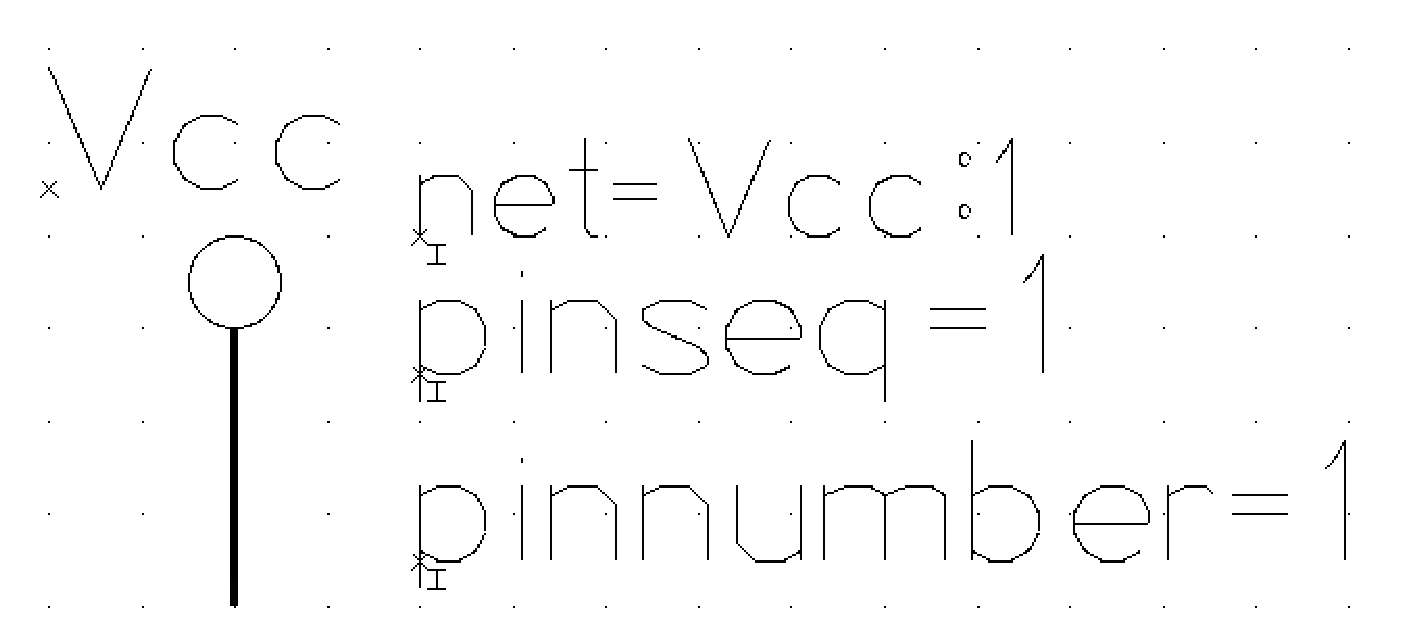
\includegraphics[clip,scale=0.2]{generic_vcc.eps}
		\caption{A power symbol with a hard-wired net attribute.  The attributes to the right of the symbol are made invisible on the schematic.\label{symbol_nonet}}
	\end{center} 
\end{figure}

\begin{figure}[ht]
	\begin{center}
		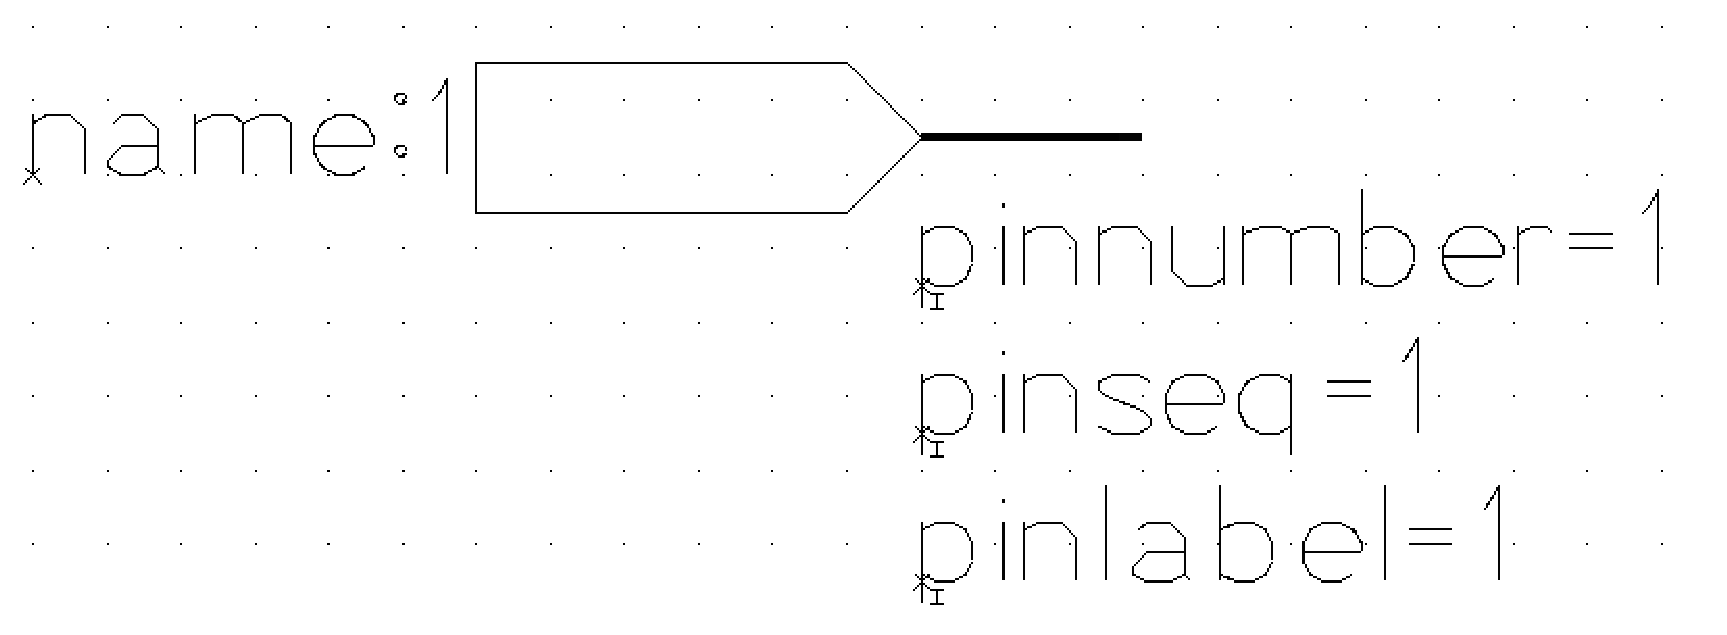
\includegraphics[clip,scale=0.2]{input_netname.eps}
		\caption{An off-page connector symbol with a net attribute you can change at the schematic level.  The attributes to the right of the symbol are made invisible on the schematic.\label{symbol_net}}
	\end{center} 
\end{figure}
